%\motto{Use the template \emph{chapter.tex} to style the various elements of your chapter content.}
\chapter{Quantensoftware und Programmierung}
\label{programming} % Always give a unique label
% use \chaptermark{}
% to alter or adjust the chapter heading in the running head

\chapterauthor{Konrad Maywald, Daniel Purtov, Dennis Schweigert, Tom Williard}

\abstract{some abstract}

\section{Programmiermodelle in der Quanteninformatik}

\subsection{Gate-basiertes Paradigma (Quantum Circuit Model)}
Das Gate basierte Paradigma oder auch Quantenschaltkreis Modell (engl. Quantum Circuit Model) genannt, ist das Standardmodell für die Programmierung von Quantenprogrammen. Daher wird es auch häufig als das am weitesten verbreitete Paradigma in der Quanteninformatik zur Beschreibung und Realisierung von Quantenalgorithmen bezeichnet. In diesem Modell werden die Quantenprogramme als Schaltkreise (engl. Quantum circuits) dargestellt. Diese bestehen aus einer Sequenz von unitären Quanten Gattern, welche auf Qubits angewendet werden. 

Strukturell orientiert sich das Quantenschaltkreismodell an klassischen digitalen Schaltungen. Klassische Schaltkreise bestehen aus Leitungen, Gattern und klassischen Bits mit den Zuständen 0 und 1. Ganz analog dazu bestehen Quantenschaltkreise aus Qubit-Leitungen und Gattern und Quantenbits (Qubits). Jede Leitung repräsentiert dabei ein Qubit und jedes Gatter eine unitäre Transformation auf eines oder mehrere Qubits. Die Struktur des Quantenschaltkreis wird genauso wie bei digitalen Schaltungen meist visuell dargestellt, um die Reihenfolge der angewendeten Operationen und die daran beteiligten Qubits zu verdeutlichen. 

Folgende Abbildung zeigt typische elementare Gates, welche für die Konstruktion von Quantenschaltkreisen verwendet, werden: 
\begin{figure}
    \centering
    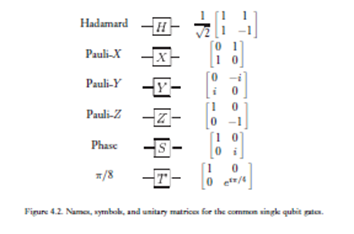
\includegraphics[width=0.5\linewidth]{Qubit Gates.png}
    \caption{Qubit Gates}
    \label{fig:enter-label}
\end{figure}

\begin{itemize}
    \item Das Hadamard-Gate (H) bringt Qubits aus Ihren Basiszuständen in eine Superposition 
    \item Das CNOT-Gate (Controlled-Not), ist ein zwei Qubit Gate, welches als zentraler Bestandteil der Quantenverschränkung funktiert, es verschränkt sozusagen zwei Qubits miteinander 
    \item Neben diesen beiden sehr wichtigen Gates gibt es auch noch die Pauli-X, -Y. und -Z Gates, sowie Phasengatter, T-Gate  und weitere 
\end{itemize}
Werden mehrerer dieser Gatter nacheinander auf ein Qubit Register angewendet, bildet sich daraus ein Quanten-Schaltkries, welcher als gesamter Algorithmus verstanden werden kann.
\subsection*{Bekannte Quantenalgorithmen basierend auf dem Quantenschaltkreismodell}
Das Quantenschaltkreismodell dient als Grundlage für mehrere bekannte Quantenalgorithmen dazu zählen folgende: (siehe auch (\autoref{basic_algorithms}))
\subsubsection*{1) Shor's Algorithmus}
Der Shor Algorithmus führt eine effiziente Primfaktorzerlegung großer Zahlen durch, was klassische Verschlüsselungsverfahren wie RSA bedroht. Der Algorithmus verwendet die Quantum Fourier Transformation (QFT) und periodenfindende Subroutinen innerhalb des Circuit-Models. (siehe auch (\autoref{first:shor-algorithm})
\subsubsection*{2) Grover´s Algorithmus}
Der Grover Algorithmus dient zur Suche eines Eintrags in einer unstrukturierten Datenbank mit einer quadratischen Beschleunigung gegenüber klassischen Verfahren.
Der Algorithmus basiert auf Rotation in einem zweidimensionalen Unterraum, dargestellt als wiederholte Anwendung von sogenannten Grover-Iterationen, realisiert durch Gates im Circuit-Modell. (ausführliche Erklärung: (\autoref{sec:grover-algorithm})) 

\subsubsection*{3) Regev}
Regevs Arbeiten zum LWE-Problem beinhalten eine theoretische Quantenreduktion, die sich vollständig im gate-basierten Modell realisieren lässt. Die dafür erforderlichen Operationen – wie das Erzeugen von Superpositionen, die Anwendung der Quanten-Fouriertransformation sowie die Verarbeitung von Messresultaten – sind mit klassischen Quanten-Gattern (z.B. Hadamard-, CNOT- und Phasengattern) darstellbar. Auch wenn Regevs Reduktion primär theoretischer Natur ist und keine praktischen Implementierungen wie Shor oder Grover hat, zeigen die verwendeten Techniken eine klare Kompatibilität mit dem Quantum Circuit Model.
\textbf{Hier muss ne Leerzeile rein geht aber nicht}
Das gate-basierte Paradigma ist nicht nur ein theoretisches Modell, das man in der Quanteninformatik zur Beschreibung von Algorithmen verwendet – es spielt auch in der Praxis eine zentrale Rolle. So setzt zum Beispiel das Open-Source-Framework Qiskit von IBM genau auf dieses Modell: Quantenprogramme werden dort direkt als sogenannte „Quantum Circuits“ aufgebaut. Diese bestehen aus einer festen Anzahl von Qubits und einer Folge von Operationen, also Gattern, Messungen und Resets – genau wie es im Schaltkreis-Modell vorgesehen ist.
Dass Theorie und Praxis hier so eng zusammenhängen, zeigt, wie wichtig das gate-basierte Modell nicht nur für die Entwicklung von Algorithmen ist, sondern auch für den praktischen Einsatz auf echten Quantencomputern, wie denen von IBM oder Google.

\subsection{Messungsbasiertes Paradigma}
\begin{itemize}
    \item Berechnung durch gezielte Messungen an verschränkten Zuständen (Cluster-States)
    \item Algorithmus wird durch Reihenfolge und Auswahl der Messungen bestimmt
    \item Beispiele:
    \begin{itemize}
        \item Teleportationsprotokoll
        \item Messungsbasierte Varianten von Grover/Shor
    \end{itemize}
\end{itemize}

\subsection{Adiabatisches Paradigma (Quantum Annealing)}
Ein weiteres Modell zur Realisierung von Quantenalgorithmen ist das adiabatische Paradigma, welches auch als Quantum Annealing bezeichnet wird. Das Adiabatischen Modell basiert auf der Idee, ein Quantensystem durch eine langsame, kontinuierliche Änderung eines Hamiltonians gezielt in seinen Grundzustand zu führen. Die gesuchte Lösung des Modells ist in diesem Grundzustand markiert. Genau in dieser Art unterscheidet sich das Quantum Annealing auch vom Gate oder messungsbasierten Modell. 
Das Grundprinzip des Modells besteht darin, dass man das Quantensystem zunächst in einem leicht vorbereiteten Anfangszustand hält. Dieser entspricht dem Grundzustand eines sogenannten Treibenden Hamiltonians $H_D$. Dieser Hamiltonian kann z.B. ein transversales Feld enthalten, das alle Qubits gleichmäßig beeinflusst. Im Laufe des Algorithmus wird dann schrittweise der Problem-Hamiltonian $H_P$ zugeschaltet, dieser enthält die Struktur des zu lösenden Problems. Die Gesamtentwicklung erfolgt über einen zeitabgängigen Hamiltonian, der folgenden Form:
$$
H(t) = A(t) \cdot H_D + B(t) \cdot H_P
$$
Die beiden Funktionen A(t) und B(t) steuern, wie stark der jeweilige Hamiltonian zu einem bestimmten Zeitpunkt t wirkt. Am Anfang dominiert hierbei HD und am Ende HP. Das System bleibt nach dem adiabatischen Theorem während des gesamten Prozesses im jeweiligen Grundzustand, wenn die Änderungen langsam genug erfolgen. Am Ende wird die gesuchte Lösung, also der Grundzustand von $H_P$ erreicht.
Die Hamiltonian dürfen mit einer Geschwindigkeit geändert werden, die stark vom sogenannten Energieabstand (Gap) zwischen dem Grundzustand und dem ersten angeregten Zustand abhängt. Je kleiner dieser Abstand ist, desto langsamer muss die Änderung erfolgen, um unerwünschte Übergänge in angeregte Zustände zu vermeiden. 
Das Quantum Annealing eignet sich besonders gut für kombinatorische Optimierungsprobleme, da viele davon auf sogenannte Ising-Modelle abgebildet werden können. Ein Beispiel für ein Problem-Hamiltonian ist folgendes:
$$
H_P = \sum_{i,j} J_{ij}\sigma_i^z\sigma_j^z + \sum_i h_i\sigma_i^z
$$
Die Kopplungsterme $J_{ij}$ und die lokalen Felder $h_i$ kodieren hierbei die jeweilige Problemstruktur.
Es gibt verschiedene Problemklassen, welche durch Quantum Annealing gelöst werden können, zu den typischen gehören unter anderem Folgende Beispiele: 
\begin{itemize}
    \item \textbf{Max-Cut: }Bei Max-Cut wird ein Graph aufgeteilt in zwei Teilmengen, sodass die Kantensumme zwischen den beiden Mengen maximal wird 
    \item 	\textbf{k-Clique:} Bei der k-Clique-Suche geht es darum, vollständige Teilgraphen mit genau k Knoten zu finden, also Untergruppen, in denen jeder Knoten mit jedem anderen verbunden ist 
    \item \textbf{Graph Coloring: }Beim Graph Coloring sollen Knoten eines Graphen mit möglichst wenigen Farben so eingefärbt werden, dass benachbarte Knoten unterschiedliche Farben erhalten 
    \item \textbf{Ising-Modell-Minimierung:} Hier wird der Ising-Hamiltonian direkt minimiert. Da sich viele kombinatorische Probleme darauf abbilden lassen, bildet diese Minimierung die Grundlage für zahlreiche Optimierungsaufgaben 
\end{itemize}
Quantum Annealing (QA) verwendet im Gegensatz zum klassischen Simulated Annealing (SA), bei der thermische Fluktuationen benutzt werden, Quantenfluktuationen, insbesondere Quanten-Tunnel, um Energiebarrieren zu überwinden. Das ist vor allem dann ein Vorteil, wenn die Energiebarrieren hoch, aber schmal sind. In genau diesen Fällen kann das Quantum Annealing schneller zu einer optimalen Lösung finden als sein klassischen Gegenstück Simulated Annealing. 
Das adiabatische Paradigma wurde in der Praxis unter anderem durch die Firma D-Wave Systems in Hardware umgesetzt. Die Systeme von D-Wave Systems sind darauf spezialisiert Optimierungsprobleme durch Quantum Annealing zu lösen, also das adiabatische Paradigma technisch zu realisieren. 
\subsection{Hybrid-Paradigma}
\begin{itemize}
    \item Kombination klassischer und quantenbasierter Teilalgorithmen
    \item Klassischer Teil optimiert, evaluiert oder trainiert Quantenschaltungen
    \item Beispiele:
    \begin{itemize}
        \item Variational Quantum Eigensolver (VQE)
        \item Quantum Approximate Optimization Algorithm (QAOA)
        \item Quantum Machine Learning (QML)
    \end{itemize}
\end{itemize}

\subsection{Funktionelles Paradigma}
\begin{itemize}
    \item Quantenprogramme als Funktionen (ähnlich funktionaler Programmierung)
    \item Häufig genutzt in Theorie und formaler Verifikation
    \item Beispiele: 
    \begin{itemize}
        \item Formalisierte Algorithmen (z.\,B. Shor, Grover)
        \item Verifizierte Protokolle (z.\,B. Superdense Coding)
        \item Einsatz linearer Typ-Systeme zur Abbildung von Quanteneigenschaften
    \end{itemize}
\end{itemize}

\section{Quanten-Programmiersprachen und -Frameworks}
\label{sec:programming-languages}


Die Entwicklung von Quantencomputern hat zur Entstehung spezialisierter Programmiersprachen und Frameworks geführt, die die besonderen Eigenschaften des Quantencomputings berücksichtigen. Diese Sprachen und Frameworks ermöglichen es Entwicklern, Quantenalgorithmen zu implementieren und zu testen, ohne sich mit den komplexen physikalischen Details der Quantenhardware auseinandersetzen zu müssen.

Im Gegensatz zu klassischen Programmiersprachen müssen Quanten-Programmiersprachen spezielle Konzepte wie Superposition, Verschränkung und Messung unterstützen. Sie müssen auch die Interaktion zwischen klassischen und Quantenberechnungen ermöglichen, da die meisten Quantenalgorithmen sowohl klassische als auch Quantenkomponenten enthalten.

Dieses Kapitel gibt einen Überblick über die verschiedenen Arten von Quanten-Programmiersprachen und ordnet sie den vorangegangenen Programmierparadigmen zu. Anschließend werden drei wichtige Frameworks - Qiskit von IBM, Cirq von Google und Q\# von Microsoft - detailliert betrachtet.

\subsection{Übersicht über Sprachen und Frameworks}


\begin{itemize}
    \item Quanten-Programmiersprachen lassen sich in verschiedene Kategorien einteilen:
    \begin{itemize}
        \item \textbf{Imperative Quanten-Programmiersprachen}
        \begin{itemize}
            \item Basieren auf Statements, die den globalen Zustand eines Programms ändern
            \item Verwenden das QRAM-Modell (Quantum Random Access Machine)
            \item Beispiele: QCL, LanQ, qGCL
        \end{itemize}
        
        \item \textbf{Funktionale Quanten-Programmiersprachen}
        \begin{itemize}
            \item Basieren auf mathematischen Transformationen durch Ausführung von Abbildungen
            \item Verwenden Lambda-Kalkül und oft lineare Logik
            \item Beispiele: QFC, QPL, QML
        \end{itemize}
        
        \item \textbf{Hybride Ansätze}
        \begin{itemize}
            \item Kombinieren klassische und Quantenprogrammierung
            \item Ermöglichen komplexe Interaktionen zwischen klassischen und Quantenalgorithmen
            \item Beispiele: Q\#, Qiskit, Cirq
        \end{itemize}
    \end{itemize}
\end{itemize}

\begin{itemize}
    \item \textbf{Industriegetriebene Frameworks}
    \begin{itemize}
        \item \textbf{Qiskit (IBM)}
        \begin{itemize}
            \item Open-Source-SDK für Quanteninformatik
            \item Python-basiert
            \item Unterstützt IBM Quantum Experience Hardware
            \item Umfangreiches Ökosystem von Tools und Plugins
        \end{itemize}
        
        \item \textbf{Cirq (Google)}
        \begin{itemize}
            \item Open-Source-Framework für Quantencomputing
            \item Python-basiert
            \item Optimiert für Google's Quantenprozessoren
            \item Fokus auf rauschbewusste Simulationen
        \end{itemize}
        
        \item \textbf{Q\# (Microsoft)}
        \begin{itemize}
            \item Eigenständige domänenspezifische Sprache
            \item Teil des Microsoft Quantum Development Kit
            \item Fokus auf Algorithmusdefinition statt Schaltkreisdarstellung
            \item Starke Typisierung und symbolische Codemanipulation
        \end{itemize}
        
        \item \textbf{PyQuil (Rigetti)}
        \begin{itemize}
            \item Python-Bibliothek für Quantenprogrammierung
            \item Zugriff auf Rigetti's Quantum Cloud Services
            \item Basiert auf Quil (Quantum Instruction Language)
        \end{itemize}
    \end{itemize}
    
    \item \textbf{Akademische und Open-Source-Frameworks}
    \begin{itemize}
        \item \textbf{Quipper}
        \begin{itemize}
            \item Eingebettet in Haskell
            \item Stark typisierte, funktionale Quantenprogrammiersprache
        \end{itemize}
        
        \item \textbf{Scaffold/ScaffCC}
        \begin{itemize}
            \item Eingebettet in C/C++
            \item Nutzt die LLVM-Infrastruktur
        \end{itemize}
        
        \item \textbf{QWire}
        \begin{itemize}
            \item Eingebettet in das Beweissystem Coq
        \end{itemize}
        
        \item \textbf{ProjectQ}
        \begin{itemize}
            \item Open-Source-Framework in Python
            \item Fokus auf Schaltkreisoptimierung und -manipulation
        \end{itemize}
    \end{itemize}
\end{itemize}

\begin{itemize}
    \item \textbf{Gate-basiert:} Qiskit (IBM), Cirq (Google)
    \item \textbf{Adiabatisch:} D-Wave Ocean SDK
    \item \textbf{Hybrid:} PennyLane, TensorFlow Quantum, Qiskit (Variational Circuits)
    \item \textbf{Funktionell / Linear:} Quipper, Q\#, Proto-Quipper, QML
\end{itemize}
-> Ergänzung um weitere und Darstellung als Tabelle

\subsection{Vertiefung ausgewählter Frameworks}
\begin{itemize}
    \item \textbf{Qiskit SDK:} Umfangreiche Bibliotheken, Simulator, Backendsteuerung
    \item \textbf{Cirq:} Framework von Google für Schaltungsdesign und Simulation
    \item \textbf{Q\#:} Domänenspezifische Sprache von Microsoft
    \item (\textbf{Quipper, Qrisp, OpenQL, Sliq:} Alternativen für High-Level- oder domänenspezifisches Design)
\end{itemize}

\subsubsection{Qiskit}
Architktur
\begin{itemize}
    \item \textbf{Mehrschichtige Architektur}
    \begin{itemize}
        \item \textbf{Terra}: Grundlegende Funktionalität für das Arbeiten mit Quantenschaltkreisen
        \begin{itemize}
            \item Schaltkreisdarstellung und -manipulation
            \item Transpiler für Optimierung und Übersetzung
            \item Backend-Schnittstellen für Simulation und Hardware-Ausführung
        \end{itemize}
        
        \item \textbf{Aer}: Hochleistungs-Simulatoren
        \begin{itemize}
            \item Unterstützt verschiedene Simulationstypen: Zustandsvektor, Dichtematrix, Stabilisator
            \item Ermöglicht Rauschsimulation
        \end{itemize}
        
        \item \textbf{Ignis}: Werkzeuge für Charakterisierung und Fehlerminderung
        \begin{itemize}
            \item Fehlercharakterisierung und -kalibrierung
            \item Fehlerminderungstechniken
        \end{itemize}
        
        \item \textbf{Aqua}: Algorithmen für verschiedene Anwendungsbereiche
        \begin{itemize}
            \item Chemie, Finanzen, Maschinelles Lernen, Optimierung
        \end{itemize}
    \end{itemize}
    
    \item \textbf{Abstrakte und konkrete Schaltkreise}
    \begin{itemize}
        \item Abstrakte Schaltkreise: Repräsentation von Quantenalgorithmen auf hoher Abstraktionsebene
        \item Konkrete Schaltkreise: Implementierung mit Standardbibliothek von Gates
        \item OpenQASM als Zwischensprache für Quantenschaltkreise
    \end{itemize}
    
    \item \textbf{Transpiler}
    \begin{itemize}
        \item Übersetzt und optimiert Schaltkreise für die Ziel-Hardware
        \item Arbeitet in mehreren Durchläufen mit verschiedenen Passes
        \item Wichtige Passes:
        \begin{itemize}
            \item Layout-Selektion: Mapping von logischen zu physischen Qubits
            \item Routing: Einfügen von SWAP-Gates für nicht direkt verbundene Qubits
            \item Optimierung: Zusammenfassen von Gates, Entfernen unnötiger Gates
            \item Dekomposition: Zerlegung komplexer Gates in elementare Gates
        \end{itemize}
    \end{itemize}
    
    \item \textbf{Primitives}
    \begin{itemize}
        \item Grundlegende Bausteine für Quantenberechnungen
        \item \texttt{Sampler}: Stichproben aus Quantenschaltkreisen ziehen
        \item \texttt{Estimator}: Erwartungswerte von Observablen schätzen
    \end{itemize}
\end{itemize}

Besonderheiten und Anwendung

\begin{itemize}
    \item \textbf{Dynamische Schaltkreise}
    \begin{itemize}
        \item Ermöglichen klassisch kontrollierte Quantenoperationen
        \item Unterstützen Mid-Circuit-Messungen und bedingte Operationen
        \item Wichtig für adaptive Algorithmen und Fehlerkorrektur
    \end{itemize}
    
    \item \textbf{Fehlerminderung}
    \begin{itemize}
        \item Verschiedene Techniken zur Reduzierung von Hardwarefehlern
        \item Zero-Noise Extrapolation
        \item Probabilistic Error Cancellation
        \item Dynamical Decoupling
    \end{itemize}
    
    \item \textbf{Anwendungsgebiete}
    \begin{itemize}
        \item Quantenchemie und Materialwissenschaft
        \item Optimierungsprobleme
        \item Maschinelles Lernen
        \item Finanzmathematik
    \end{itemize}
    
    \item \textbf{Ökosystem und Community}
    \begin{itemize}
        \item Über 6 Millionen Installationen, 300.000 pro Monat
        \item 500+ Mitwirkende, die meisten nicht von IBM
        \item 300+ Pakete im Python Package Index (PyPI) hängen von Qiskit ab
        \item Über 2.000 wissenschaftliche Arbeiten haben Qiskit verwendet
    \end{itemize}
\end{itemize}

\subsubsection{Cirq}
Achitektur
\begin{itemize}
    \item \textbf{Grundlegende Abstraktionen}
    \begin{itemize}
        \item \texttt{Qubit}: Repräsentation eines Quantenbits
        \item \texttt{Gate}: Quantenoperationen auf Qubits
        \item \texttt{Circuit}: Sequenz von Quantenoperationen
        \item \texttt{Moment}: Sammlung von Operationen, die parallel ausgeführt werden können
    \end{itemize}
    
    \item \textbf{Hardware-spezifische Optimierung}
    \begin{itemize}
        \item Speziell für Google's Quantenprozessoren optimiert
        \item Berücksichtigt Hardware-Topologie und -Einschränkungen
        \item Unterstützt aber auch andere Hardware-Plattformen
    \end{itemize}
    
    \item \textbf{Rauschmodellierung}
    \begin{itemize}
        \item Fortschrittliche Werkzeuge zur Simulation von Rauschen
        \item Verschiedene Rauschmodelle für realistische Simulationen
        \item Ermöglicht die Untersuchung der Auswirkungen von Rauschen auf Quantenalgorithmen
    \end{itemize}
    
    \item \textbf{Python-Integration}
    \begin{itemize}
        \item Tiefe Integration mit dem Python-Ökosystem
        \item Kompatibel mit NumPy, SciPy und anderen wissenschaftlichen Bibliotheken
        \item Ermöglicht die Nutzung bestehender Python-Tools für Datenanalyse und Visualisierung
    \end{itemize}
\end{itemize}

Besonderheiten
\begin{itemize}
    \item \textbf{Kalibrierungswerkzeuge}
    \begin{itemize}
        \item Werkzeuge zur Kalibrierung von Quantenhardware
        \item Optimierung der Gateoperationen für spezifische Hardware
        \item Wichtig für die praktische Implementierung von Quantenalgorithmen
    \end{itemize}
    
    \item \textbf{Fokus auf NISQ-Ära}
    \begin{itemize}
        \item Optimiert für Noisy Intermediate-Scale Quantum (NISQ) Computer
        \item Unterstützt Algorithmen, die mit begrenzter Qubit-Anzahl und Fehlerraten arbeiten können
        \item Variational Quantum Eigensolver (VQE)
        \item Quantum Approximate Optimization Algorithm (QAOA)
    \end{itemize}
    
    \item \textbf{Visualisierungswerkzeuge}
    \begin{itemize}
        \item Umfangreiche Werkzeuge zur Visualisierung von Quantenschaltkreisen
        \item Analyse von Simulationsergebnissen
        \item Darstellung von Quantenzuständen und -operationen
    \end{itemize}
    
    \item \textbf{Anwendungsgebiete}
    \begin{itemize}
        \item Quantenmaschinelles Lernen
        \item Quantenchemie
        \item Optimierungsprobleme
        \item Grundlagenforschung in der Quanteninformatik
    \end{itemize}
\end{itemize}

\subsubsection{Q\#}
Architektur
\begin{itemize}
    \item \textbf{Eigenständige domänenspezifische Sprache}
    \begin{itemize}
        \item Nicht eingebettet in eine klassische Sprache
        \item Speziell für Quantencomputing entwickelt
        \item Teil des Microsoft Quantum Development Kit
    \end{itemize}
    
    \item \textbf{Typsystem}
    \begin{itemize}
        \item Starke Typisierung
        \item Betont klassischen Determinismus
        \item First-Class-Callables (Funktionen als Werte)
        \item Opazität von Qubit-Typen (keine direkten Zugriffe auf Qubit-Zustände)
    \end{itemize}
    
    \item \textbf{Kontrollstrukturen}
    \begin{itemize}
        \item Klassische Kontrollstrukturen: if/else, for, while
        \item Quantenspezifische Kontrollstrukturen: repeat-until-success
        \item Unterstützung für rekursive Algorithmen
    \end{itemize}
    
    \item \textbf{Symbolische Codemanipulation}
    \begin{itemize}
        \item Automatische Generierung des Adjungierten (konjugiert transponierte) einer Operation
        \item Kontrollierte Versionen von Operationen
        \item Funktioniert auf Typ-Ebene, nicht nur auf Wert-Ebene
    \end{itemize}
\end{itemize}
Besonderheiten
\begin{itemize}
    \item \textbf{Klare Trennung von Quantencode und klassischem Code}
    \begin{itemize}
        \item Quantencode wird in Q\# geschrieben
        \item Klassischer Treibercode kann in C\#, Python oder anderen Sprachen geschrieben werden
        \item Saubere Schnittstelle zwischen beiden Welten
    \end{itemize}
    
    \item \textbf{Fokus auf Algorithmusdefinition}
    \begin{itemize}
        \item Q\# ist eine Algorithmusdefinitionssprache, keine Schaltkreisbeschreibungssprache
        \item Natürliche Darstellung der Komposition von klassischen und Quantenalgorithmen
        \item Kein explizites Konzept eines "Schaltkreises"
    \end{itemize}
    
    \item \textbf{Unterstützung für komplexe Algorithmen}
    \begin{itemize}
        \item Besonders geeignet für Phasenabschätzung und Quantenchemie-Algorithmen
        \item Unterstützt reichhaltige Quantenklassische Interaktionen
        \item Ermöglicht die Erstellung von Algorithmen mit nicht-trivialem Branching
    \end{itemize}
    
    \item \textbf{Simulation und Ressourcenschätzung}
    \begin{itemize}
        \item Verschiedene Simulatoren für unterschiedliche Zwecke
        \item Werkzeuge zur Schätzung der benötigten Ressourcen (Qubits, Gates)
        \item Wichtig für die Entwicklung skalierbarer Quantenalgorithmen
    \end{itemize}
    
    \item \textbf{Anwendungsgebiete}
    \begin{itemize}
        \item Quantenkryptographie
        \item Quantenchemie
        \item Optimierungsprobleme
        \item Fehlerkorrektur und fehlertolerantes Quantencomputing
    \end{itemize}
\end{itemize}

\section{Entwicklung von Quantenalgorithmen}

\subsection{Überblick über den Entwicklungsprozess}
\begin{itemize}
    \item Ziel: Praktische Umsetzung eines Quantenalgorithmus (End-to-End)
    \item Typische Phasen:
    \begin{itemize}
        \item Problemformulierung (z.\,B. Suche, Optimierung, Simulation)
        \item Auswahl eines geeigneten Paradigmas
        \item Abbildung auf ein Quantenmodell
        \item Wahl geeigneter Sprache / Frameworks (z.\,B. Qiskit)
        \item Implementierung, Testing, Ausführung (lokal und cloudbasiert)
    \end{itemize}
\end{itemize}

\subsection{Quantum Software Stack}

Das Quantencomputing basiert auf einem mehrschichtigen Software-Stack, mit dem abstrakte Quantenalgorithmen auf Quantenhardware übertragen und ausgeführt werden können. Eine mögliche Strukturierung eines solchen Software-Stacks ist in \autoref{fig:quantum-software-stack} abgebildet und setzt sich aus den drei Ebenen \emph{Nutzer (User Layer)}, \emph{Plattform (Platform Layer)} und \emph{Hardware (Hardware Layer)} zusammen. Jede dieser Schichten übernimmt spezifische Aufgaben innerhalb des Gesamtsystems und abstrahiert die Komplexität der darunterliegenden Ebenen.
\\
\paragraph{Nutzer}  
In der obersten Schicht werden Problemstellungen mittels Quantenalgorithmen (\autoref{basic_algorithms}) in konkreten Anwendungscode übertragen. Sie umfasst Werkzeuge und Bibliotheken, mit denen Entwickler Quantenalgorithmen und -anwendungen implementieren und für die Ausführung auf Quantenhardware vorbereiten können. Dazu gehören vor allem die in \autoref{sec:programming-languages} näher erläuterten Programmiersprachen und Entwicklungswerkzeuge (SDKs und Frameworks) wie Qiskit, Cirq oder Q\#.
\\
\paragraph{Plattform}  
Die Plattformschicht ist für die Kompilierung und Optimierung von Quantenprogrammen zuständig. Dazu gehören Compiler wie TKET oder der Qiskit Transpiler, die den Programmcode in Quantenhardware-kompatible Befehle übersetzen. Dazu zählen z.B. Gate-Dekomposition, Qubit-Zuordnung und Optimierung hinsichtlich Laufzeit und Fehlerresistenz. Auch dedizierte Software zur Fehlerkorrektur wie Riverlane kann dieser Schicht zugeordnet werden. Darüber hinaus enthält die Plattformschicht Simulatoren und Emulatoren wie Qiskit Aer oder Intel Quantum Simulator. Dabei handelt es sich um Software, die echte Quantenhardware nachbildet und so ein einfacheres Testen, Debuggen und Optimieren von Quantenanwendungen ermöglicht.
\\
\paragraph{Hardware}  
Am unteren Ende des Software-Stacks befindet sich die eigentliche Quantenhardware (Quantum Processing Unit) sowie Software für deren Verwaltung und Überwachung. Kontrollsysteme wie Quantum Machines OPX+ ermöglichen beispielsweise die Kalibrierung, Pulsgenerierung und qubitgenaue Steuerung der Hardware. Außerdem umfasst die Hardwareschicht weitere Fehlerkorrekturmechanismen.
\\
\\
Jede Schicht im Software-Stack abstrahiert technische Details der darunterliegenden Ebene und trägt zur strukturierten Entwicklung, Optimierung und Ausführung von Quantenprogrammen bei. \autocite{shehata_building_2025} \autocite{ryan_understanding_2024}

\begin{figure}[ht!]
\centering
\begin{tikzpicture}[
  layerbox/.style={
    draw,
    minimum width=6cm,
    minimum height=0.8cm,
    text centered
  }
]

\node[layerbox] (l1) at (0,  0) {Programmiersprachen};
\node[layerbox] (l2) at (0, -1) {SDKs und Frameworks};
\node[layerbox] (l3) at (0, -2) {Quantenalgorithmen};
\node[layerbox] (l4) at (0, -3) {Quantenanwendungen};

\node[layerbox] (l5) at (0, -4.5) {Simulation};
\node[layerbox] (l6) at (0, -5.5) {Kompilierung};
\node[layerbox] (l7) at (0, -6.5) {Fehlerkorrektur};

\node[layerbox] (l8) at (0, -8) {Kontrollsysteme};
\node[layerbox] (l9) at (0, -9) {Quantum Processing Unit (QPU)};

\draw[decorate, decoration={brace, amplitude=6pt, mirror}, very thick]
  ($(l1.north west) + (-0.2,0.1)$) -- ($(l4.south west) + (-0.2,-0.1)$)
  node[midway, xshift=-0.4cm, anchor=east, font=\normalsize\bfseries] {Nutzer};

\draw[decorate, decoration={brace, amplitude=6pt, mirror}, very thick]
  ($(l5.north west) + (-0.2,0.1)$) -- ($(l7.south west) + (-0.2,-0.1)$)
  node[midway, xshift=-0.4cm, anchor=east, font=\normalsize\bfseries] {\textbf{Plattform}};

\draw[decorate, decoration={brace, amplitude=6pt, mirror}, very thick]
  ($(l8.north west) + (-0.2,0.1)$) -- ($(l9.south west) + (-0.2,-0.1)$)
  node[midway, xshift=-0.4cm, anchor=east, font=\normalsize\bfseries] {\textbf{Hardware}};

\end{tikzpicture}
\caption{Struktur eines Quantum Software-Stacks \autocite{ryan_understanding_2024}}
\label{fig:quantum-software-stack}
\end{figure}

\textbf{Näher eingehen auf Compiler und Simulator?}

\subsection{Quantum Cloud Computing}

Die in der untersten Schicht des Quantum Software-Stacks befindliche Quantenhardware ist teuer in der Anschaffung und komplex zu betreiben. Das Konzept des Quantum Cloud Computing (QCC) zielt darauf ab, Endnutzern den Zugang zu Quantenhardware über Cloud-Plattformen zu erleichtern. Diese bieten Zugang zu Ressourcen, Jobmanagement und Fehlermitigation mittels abstrahierter Schnittstellen in einer skalierbaren Umgebung.

Ein zentraler Vorteil Cloud-basierter Quantenplattformen liegt in ihrer Flexibilität: Nutzer können ihre Rechenkapazitäten bedarfsgerecht skalieren, was die Bearbeitung unterschiedlich komplexer Probleme effizienter gestaltet. Außerdem ermöglichen sie das einfache Entwickeln und Testen von Quantenalgorithmen in simulierten Umgebungen, bevor diese auf echter Hardware ausgeführt werden. Dies reduziert die Einstiegshürden, da keine spezialisierte Infrastruktur oder tiefgreifende Hardwarekenntnisse notwendig sind. Da alle Nutzer auf dieselbe Plattform zugreifen, werden darüber hinaus globale Kollaboration und standardisierte Entwicklungsumgebungen begünstigt.

Zu den wichtigsten Anbietern von Quantum Cloud Plattformen zählen aktuell IBM, Amazon und Google. Ihre Plattformen IBM Quantum\footnote{IBM Quantum \url{https://quantum.ibm.com/}}, Amazon Braket\footnote{Amazon Braket \url{https://aws.amazon.com/braket/}} und Google Quantum AI\footnote{Google Quantum AI \url{https://quantumai.google/cirq/google/concepts}} sind in \autoref{tab:quantum-cloud-platforms} gegenübergestellt \autocite{trends+challenges-TODO-sync}.

\begin{table}[ht!]
\centering
\begin{tabular}{|p{2.8cm}|p{2.5cm}|p{2.5cm}|p{4.5cm}|p{3.5cm}|}
\hline
\textbf{Plattform} & \textbf{Hardware} & \textbf{Sprachen / SDKs} & \textbf{Kernfeatures} & \textbf{Besonderheiten} \\
\hline
IBM Quantum & Falcon, Eagle (Supraleitende Qubits) & Qiskit & Hardware-agnostischer Code, Qiskit Runtime für containerisierte Near-time-Execution, integrierte Fehlerunterdrückung (z.\,B. ZNE, dynamical decoupling) & Sessions zur Reduktion klassisch-quantischer Latenz; optimiert für iterative Algorithmen \\
\hline
Amazon Braket & IonQ (Ionenfallen), Rigetti (supraleitend), OQC (Photonik) & Braket SDK, PennyLane, Qiskit & Hybrid Jobs: Orchestrierung von QPU und EC2, Priorisierung, parametric compilation, CloudWatch Monitoring & Pay-as-you-go-Modell; lokale Debug-Modi; EC2-Integration für hybride Workflows \\
\hline
Google Quantum AI & Sycamore (supraleitend) & Cirq & Integration mit Google-Infrastruktur, Fokus auf NISQ-Algorithmen und ML & Direkte ML-Pipeline-Anbindung; Forschungsfokus auf Skalierbarkeit \\
\hline
\end{tabular}
\caption{Vergleich führender Quantum Cloud Plattformen}
\label{tab:quantum-cloud-platforms}
\end{table}

Weitere Plattformen sind etwa \textit{Strangeworks}, \textit{Xanadu}, \textit{Quantinuum}, \textit{IonQ} (auch über Azure Quantum) und \textit{Microsoft Azure Quantum}. Diese bieten entweder eigene Hardwaretechnologien (wie photonische QPUs bei Xanadu oder trapped-ion Systeme bei Quantinuum) oder bündeln übergreifende Multi-Backend-Zugänge mit einheitlicher API. Microsoft ermöglicht zudem tiefe Integration in klassische Azure-Dienste, während Strangeworks auf eine benutzerfreundliche Multi-Vendor-Umgebung setzt.










\subsection{Praxisbeispiel: Grover-Suche mit Qiskit} (erledigt, nur noch beschreiben was passiert)
\begin{itemize}
    \item Ziel: Implementierung einer Grover-Suche zum Finden eines markierten Eintrags
    \item Problemformulierung und Zielzustand
    \item Bezug zur Theorie: siehe Kapitel \textit{Quantenalgorithmen}
    \item Auswahl: Gate-basiertes Modell mit Qiskit SDK
\end{itemize}

\subsection{Implementierung und Testing mit Qiskit}
\subsubsection{Projektstruktur und Setup (Python-Umgebung, Qiskit-Installation)} (erledigt)
\begin{itemize}
        \item Systemanforderungen
        \begin{table}[h]
        \centering
        \begin{tabular}{|l|l|}
        \hline
        \textbf{Komponente} & \textbf{Beschreibung} \\
        \hline
            Betriebssystem& Windows 10 oder 11 (64-Bit)\\\hline
            Python-Verson& Python 3.8 bis 3.11\\\hline
            Arbeitsspeicher& mind. 4 Gb RAM (empfohlen: 8GB oder mehr)\\
        \hline
 Festplattenspeicher &ca. 1-2GB freier Speicherplatz\\\hline
 Internetverbindung&Für Installation, Updates und optionalen IBM-Zugriff\\ \hline
        \end{tabular}
        \caption{Systemsetup für Qiskit-Projekt}
        \label{tab:setup}
\end{table}
        \item Virtuelle Umgebung einrichten und aktivieren
        \item Qiskit installieren
    \end{itemize}
\subsubsection{Konstruktion des Circuits: Dennis}


Um den Grover Algorithmus praktisch auf eine Quantencomputer umzusetzen, wird eine konkrete Konstruktion der Schaltung benötigt. Der Algorithmus setzt sich dabei aus 4 wesentlichen Komponenten zusammen: 
\begin{enumerate}
    \item  Initialisierung: Hierbei werden die Qubits in eine gleichmäßige Superposition gebracht
    \item Oracle: Im Oracle wird der gesuchte Zustand, welcher der Grover Algorithmus identifizieren soll, ausgewählt
    \item Diffusionsoperator: Der Diffusionsoperator verstärkt den Zustand des Oracle
    \item   Messung: Abgeschlossen wird der Algorithmus mit der Messung, um das Ergebnis zu erhalten. 
\end{enumerate}

Diese 4 Schritte können beliebig für eine beliebige Anzahl an Qubits angewendet werden. Im Folgenden werden die 4 Komponenten nochmals ausführlicher beschrieben. Das Ganze erfolgt jeweils mathematisch, konzeptionell und zusätzlich noch praktisch. Für den praktischen Teil wurde ein Grover Algorithmus mit Qiskit in Jupyter Notebooks implementiert und Codeausschnitte zeigen Schritt für Schritt die praktische Umsetzung.

\subsection*{Initialisierung}
Der Startzustand aller Qubits ist $\ket{0}$. Um eine gleichverteilte Superposition über alle Basiszustände der Qubits zu erzeugen, muss für jedes der Qubits ein Hadamard-Gate ($H$) angewendet werden. Für die Anzahl $n$ Qubits ergibt sich daraus folgender Zusammenhang:
$$
|\psi_0\rangle = H^{\otimes n}|0\rangle^{\otimes n} = \frac{1}{\sqrt{2^n}} \sum_{x=0}^{2^n-1} |x\rangle
$$
Der beschriebene Zustand bildet die Grundlage für die Amplitudenverstärkung von Grovers Algorithmus. Jede Lösung hat damit zunächst dieselbe Wahrscheinlichkeit. (Nielsen \& Chuang 2010, S.257)

Mit Qiskit in Jupyter Notebooks wird zunächst die `QuantumCircuit`-Bibliothek benötigt. Anschließend kann die Initialisierung, also der Ausgangspunkt für jeden Grover-Algorithmus, wie folgt in Qiskit umgesetzt werden:
\subsection*{Beispiel für 2 Qubits:}
\begin{verbatim}
from qiskit import QuantumCircuit

# Quantenschaltung mit 2 Qubits und 2 klassischen Bits erstellen
qc = QuantumCircuit(2, 2)

# Hadamard-Gate auf jedes Qubit anwenden
qc.h([0, 1])


\end{verbatim}
Das gewählte Beispiel ist für 2 Qubits, kann jedoch, wie bereits erwähnt, für die Anzahl $n$ Qubits beliebig erweitert werden.

\subsection*{Oracle}
Der nächste Schritt in der Implementierung des Grover-Algorithmus nennt sich Oracle. Bei Oracle handelt es sich um eine unitäre Operation $U_f$, welche den gesuchten Zustand $\ket{T}$ durch eine Phaseninversion der Qubits kenntlich macht. Das bedeutet, dass in diesem Schritt immer der gesuchte Zielzustand markiert wird. Dies erlaubt im Beispiel von 2 Qubits vier verschiedene Zielzustände: "00", "01", "10" und "11".

Dieser Zusammenhang wird wie folgt beschrieben:
$$
U_f \ket{x} = (-1)^{f(x)} \ket{x}
$$
Ein ideales Oracle wird formal wie folgt beschrieben:
$$
U_f \ket{x} = \begin{cases} -\ket{x} & \text{wenn } x \text{ der gesuchte Zustand ist} \\ \ket{x} & \text{sonst} \end{cases}
$$
Für die Standardversion des Grover-Algorithmus wird der Parameter $f(x)$ in der genannten Formel gesetzt, was zu folgender Formel führt:
$$
U_f \ket{x} = (-1)^{\delta_{x,T}} \ket{x}
$$
Die daraus entstehende Inversion lässt sich als eine Reflexion des Zustandsvektors im sogenannten Hilbertraum interpretieren. (Roy et al 2022, Grover 1996)

Zum besseren Verständnis, wie das Genannte mit Qiskit in Jupyter Notebooks umgesetzt wird, hier die Fortsetzung des Beispiels für 2 Qubits. Als Beispiel wird im Folgenden nun der Zielzustand $\ket{01}$ markiert.

Standardmäßig wirkt das CZ-Gate (Controlled-Z Gate) in Qiskit auf den Zustand $\ket{11}$. Wenn man nun einen der anderen genannten Zustände markieren möchte, muss man mit NOT-Gates (X-Gates) arbeiten, welche die Qubits so transformieren, dass der gewünschte Zielzustand vor dem CZ-Gate zum Zustand $\ket{11}$ wird und nach dem CZ-Gate wieder zurücktransformiert wird.

\subsection*{Zielzustand $\ket{01}$ markieren (Beispiel):}
Um den Zustand $\ket{01}$ zu markieren, invertieren wir das erste Qubit (Index 0) mit einem X-Gate, sodass aus $\ket{0}$ ein $\ket{1}$ wird. Das zweite Qubit (Index 1) bleibt $\ket{1}$. Somit wird aus $\ket{01}$ ein $\ket{11}$. Anschließend wenden wir das CZ-Gate an und invertieren das erste Qubit wieder zurück, um den Zustand wiederherzustellen.

\begin{verbatim}
# Oracle für den Zielzustand |01> erstellen
# Qubit 0 (links) ist 0, Qubit 1 (rechts) ist 1
# Um aus |01> ein |11> zu machen, muss Qubit 0 invertiert werden (X-Gate)

# X-Gate auf Qubit 0 anwenden (0 -> 1)
qc.x(0)
# CZ-Gate anwenden (wirkt auf |11>)
qc.cz(0, 1)
# X-Gate auf Qubit 0 zurückanwenden (1 -> 0)
qc.x(0)

# Schaltung zeichnen (optional)
# qc.draw('mpl')
\end{verbatim}
Mit dieser Vorgehensweise können beliebige Zielzustände auf einfache Weise realisiert werden, und das Ganze ohne zusätzliche Hilfs-Qubits. Das funktioniert auch für die Anzahl $n$ Qubits. (Roy et al, 2022)

---

\subsection*{Diffusionsoperator}
Der Diffusionsoperator, welcher auch häufig „Inversion about the mean“ genannt wird, verstärkt den im Oracle markierten Zielzustand, indem er alle Amplituden am Mittelwert reflektiert. Die Definition des Diffusionsoperators ist folgende:
$$
D = 2\ket{s}\bra{s} - I
$$
Dabei steht der Parameter $\ket{s}$ für den gleichverteilten Zustand. Das entspricht aus geometrischer Sicht einer Spiegelung im Hilbertraum. Genau diese Operation ist für die Verstärkung des im Oracle markierten Zielzustands verantwortlich. Nach jeder Grover-Iteration bewirkt sie eine Rotation des Zustandsvektors um einen festen Winkel im Unterraum von markierten und unmarkierten Zuständen. (vgl. Grover 1996, Montanaro 2016).

In unserem gewählten Beispiel mit 2 Qubits kann der Diffusionsoperator in Qiskit wie folgt umgesetzt werden:
\begin{verbatim}
# Diffusionsoperator
qc.h([0, 1])  # Hadamard-Gate auf alle Qubits
qc.x([0, 1])  # X-Gate auf alle Qubits
qc.cz(0, 1)  # CZ-Gate
qc.x([0, 1])  # X-Gate auf alle Qubits
qc.h([0, 1])  # Hadamard-Gate auf alle Qubits

# Schaltung zeichnen (optional)
# qc.draw('mpl')
\end{verbatim}

Optional kann das auch mit dem `GroverOperator` aus der Qiskit-Bibliothek gelöst werden. Dieser kapselt Oracle und Diffusion und wird wie folgt umgesetzt:
\begin{verbatim}
from qiskit.algorithms import GroverOperator

# Ein Oracle definieren (hier als Beispiel für |01>)
oracle_qc = QuantumCircuit(2)
oracle_qc.x(0)
oracle_qc.cz(0, 1)
oracle_qc.x(0)

# GroverOperator erstellen
grover_op = GroverOperator(oracle=oracle_qc)

# GroverOperator zur Hauptschaltung hinzufügen (optional, da er bereits die Iteration enthält)
# qc.append(grover_op, [0, 1])

# Schaltung zeichnen (optional)
# grover_op.draw('mpl')
\end{verbatim}

\subsubsection{Ausführung auf Simulator (Qiskit Aer)}
\subsubsection{Visualisierung von Schaltkreis und Ergebnissen Konrad}

Ein zentrales Anliegen beim Verständnis und bei der Vermittlung von Quantenalgorithmen ist die Möglichkeit, deren Funktionsweise nicht nur abstrakt-mathematisch, sondern auch visuell nachvollziehen zu können. Das folgende Kapitel widmet sich der Visualisierung des Grover-Algorithmus anhand zweier Implementierungen – einmal mit zwei, einmal mit drei Qubits – unter Verwendung des Qiskit-Frameworks. Sowohl der Aufbau des Quanten-Schaltkreises als auch die Messergebnisse werden grafisch dargestellt und interpretiert.

\subsection*{Visualisierung des Quantenschaltkreises}

Für beide Varianten des Grover-Algorithmus wird der jeweilige Quanten-Schaltkreis mit der Methode QuantumCircuit.draw() visualisiert. Diese Darstellung erlaubt einen direkten Einblick in den logischen Aufbau des Algorithmus, insbesondere in die Abfolge und Wirkung der verschiedenen quantenmechanischen Operationen. Die Schaltkreise bestehen jeweils aus mehreren charakteristischen Abschnitten:
\begin{itemize}
    \item \textbf{Initialisierung:} Alle Qubits werden im Zustand $\ket{0}$    vorbereitet.
    \item \textbf{Superposition:} Durch Anwendung von Hadamard-Gattern wird eine gleichmäßige Überlagerung aller möglichen Basiszustände erzeugt.
    \item \textbf{Oracle:} Eine gezielte Phaseninversion kennzeichnet den gesuchten Zustand. Dieser Schritt implementiert die sogenannte „Markierung“ des Zielzustands.
    \item \textbf{Diffusion (Grover-Operator):} In einem weiteren Schritt wird der markierte Zustand durch Interferenz verstärkt. Dies geschieht durch Spiegelung an der Mittelwertachse aller Amplituden.
    \item \textbf{Messung:} Zum Abschluss des Algorithmus erfolgt eine Messung aller Qubits.
\end{itemize}
\noindent
Die nachstehenden Codeausschnitte zeigen, wie die Schaltkreise für beide
Varianten im Notebook erzeugt und angezeigt werden:

\begin{verbatim}
circuit.draw()
\end{verbatim}

  \centering
  \begin{figure}
      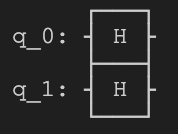
\includegraphics[width=0.25\linewidth]{circuit_superposition.png}
      \caption{Visualisierung des Schaltkreises (Superposition)}
      \label{fig:enter-label}
\end{figure}

\subsubsection*{Visualisierung der Messergebnisse}


\subsubsection{Tests und Debugging-Hilfsmittel (z.\,B. Histogramme, Counts) Konrad}



\subsection{Cloud Deployment: Ausführung auf echter Quantenhardware}

Überblick über Cloud-Plattformen für Quantenentwicklung

\begin{itemize}
    \item Vergleich führender Plattformen:
    \begin{itemize}
        \item IBM Quantum + Qiskit
        \item Amazon Braket + Braket SDK
        \item Google Quantum AI + Cirq
    \end{itemize}
    \item Zentrale Features:
    \begin{itemize}
        \item Abstraktion vom Hardware-Backend
        \item Zugang zu Simulatoren und echten Chips
        \item Ressourcenverwaltung, Warteschlangen, Fehlermitigation
    \end{itemize}
    \item Rolle innerhalb einer Entwicklungs-/Deploymentpipeline
\end{itemize}

\begin{itemize}
    \item Motivation für cloudbasierte Ausführung:
    \begin{itemize}
        \item Kein lokaler Zugang zu Quantenhardware
        \item Automatisierte Fehlerkorrektur und Abstraktion
        \item Vergleich mit klassischem Cloud Deployment
    \end{itemize}
    \item IBM Quantum:
    \begin{itemize}
        \item Account und Zugriffstoken
        \item Auswahl von Backends über Qiskit
        \item Transpilierung und Job-Submission
        \item Job-Monitoring und Ergebnisabruf
    \end{itemize}
\end{itemize}


\subsection{Tooling und Automatisierung}
\begin{itemize}
    \item Transpiler: Anpassung an spezifisches Backend
    \item Middleware: Warteschlange, Priorisierung, Job-IDs
    \item Backend-Optimierung: z.\,B. minimale Tiefe, minimale Fehlerwahrscheinlichkeit
    \item Möglichkeit automatisierter Testausführung mit Simulator
\end{itemize}

\subsection{Fazit und Ausblick}
\begin{itemize}
    \item Zusammenfassung der Entwicklungsschritte
    \item Stärken und Schwächen aktueller Toolchains
    \item Ausblick: Hybrid-Ansätze, komplexere Anwendungsfälle, Integration in klassische Softwarelandschaften
\end{itemize}

\printbibliography
